% ============================================================
%  Part 3: Applications, Limitations, and Legacy of BERT
% ============================================================

% ============================================================
%  Section: Applications of BERT
% ============================================================

\section{Applications of BERT}
\label{sec:applications}

One of \bert{}'s most significant contributions is the breadth and versatility of its
downstream applicability.  Because \bert{} is pre-trained once on massive corpora and
subsequently \emph{fine-tuned} with minimal task-specific supervision, a single
unified backbone can be adapted to a wide range of natural language processing tasks.
This section examines four representative application domains: sentiment analysis,
search intent understanding, question answering, and named entity recognition.

\subsection{Sentiment Analysis}
\label{subsec:sentiment}

Sentiment analysis---the task of classifying the emotional polarity of a piece of
text---is one of the most direct demonstrations of \bert{}'s text-classification
capability.  The input is formatted as a single sequence prefixed with the
\texttt{[CLS]} token and terminated with \texttt{[SEP]}; after fine-tuning, the
contextual representation of \texttt{[CLS]} is passed through a linear classification
head whose output dimension equals the number of sentiment classes.

Three representative examples illustrate the precision of \bert{}'s predictions.
A clearly positive review such as \emph{``I absolutely love the new product design!''}
yields a probability distribution strongly concentrated on the positive class
($P_{\text{Pos}} = 0.98$, $P_{\text{Neu}} = 0.015$, $P_{\text{Neg}} = 0.005$).
An ambiguous, informationally neutral query such as \emph{``how do I place orders''}
is correctly assigned to the neutral class ($P_{\text{Neu}} = 0.997$).  Conversely, an
implicitly negative statement such as \emph{``this is not the answer I was looking
for''} is classified as negative with high confidence ($P_{\text{Neg}} = 0.995$),
demonstrating \bert{}'s ability to capture negation through bidirectional context.
It is worth noting that \bert{}'s WordPiece tokenizer may segment rare words into
subword units prefixed with \texttt{\#\#}, but this has no adverse effect on
sentiment classification because contextual representations aggregate information
across the full token sequence~\cite{devlin2019bert}.

\subsection{Search Intent Understanding --- Google Search Integration}
\label{subsec:search}


\begin{figure}[H]
  \centering
  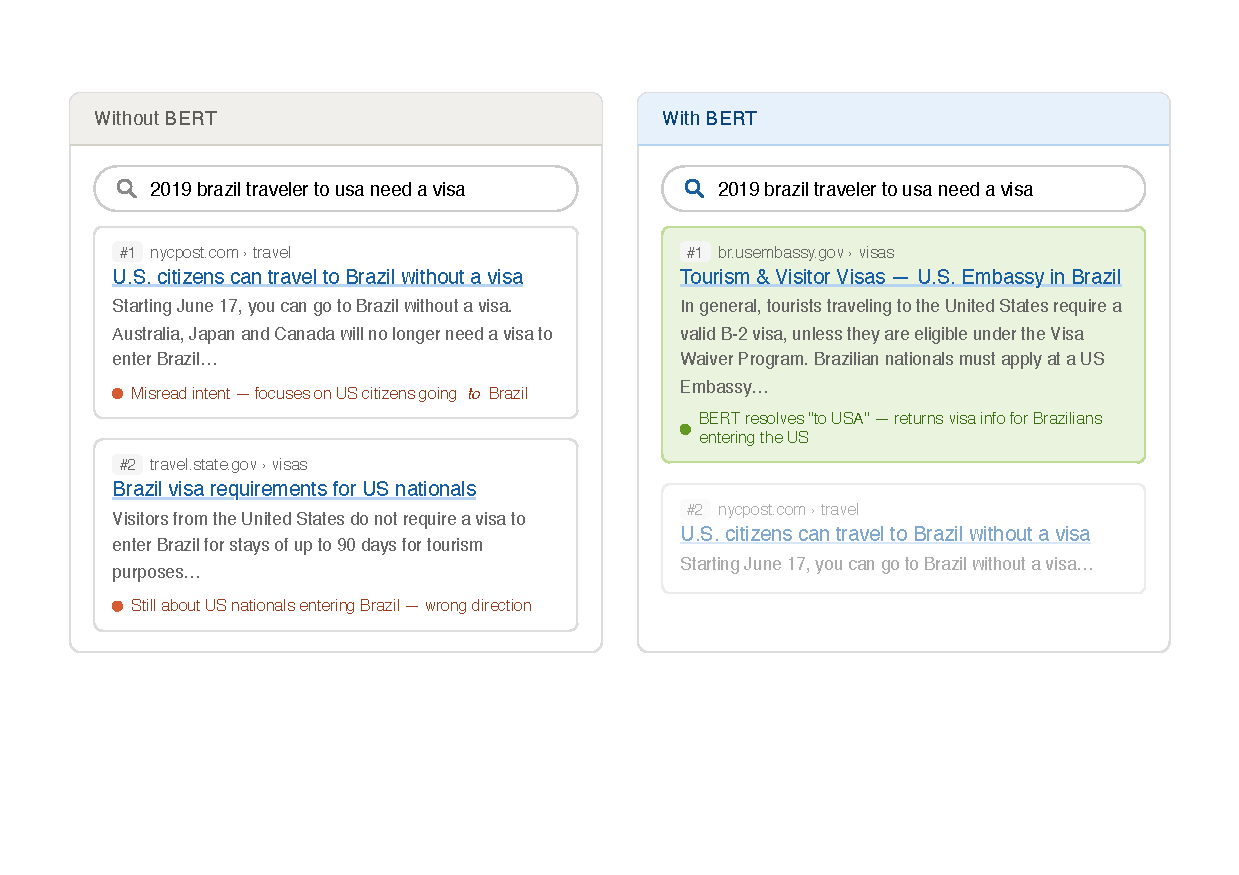
\includegraphics[trim=1cm 3.5cm 1cm 1.5cm, clip, width=0.90\textwidth]{figures/visa.pdf}
  \caption{\textbf{Impact of BERT on Search Intent Resolution.} The left panel (Without BERT) shows results focusing on U.S. citizens traveling \textit{to} Brazil, failing to capture the directional intent. The right panel (With BERT) correctly identifies the query ``2019 brazil traveler to usa'' as a request for U.S. entry requirements for Brazilian nationals.}
  \label{fig:visa-intent} % Changed to be unique and descriptive
\end{figure}

In October 2019, Google deployed \bert{} to improve the interpretation of natural
language search queries, affecting approximately one in ten English searches at
launch~\cite{nayak2019bert}.  The central challenge in web search is not merely
matching keywords but understanding the \emph{intent} embedded in a query, which
often hinges on subtle linguistic cues such as prepositions or word order.

Two canonical examples underscore this point.  For the query \emph{``2019 Brazil
traveler to USA need a visa''}, pre-\bert{} systems retrieved results focused on
US citizens travelling \emph{to} Brazil---misreading the directionality signalled by
the preposition \emph{to}.  After integrating \bert{}, the top result correctly
pointed to US Embassy visa requirements for Brazilian nationals, because \bert{}
conditions each token's representation on its full bilateral context and thus
correctly resolves the directional relationship.


\begin{figure}[H]
  \centering
  % trim= left bottom right top (adjust these values to zoom more/less)
  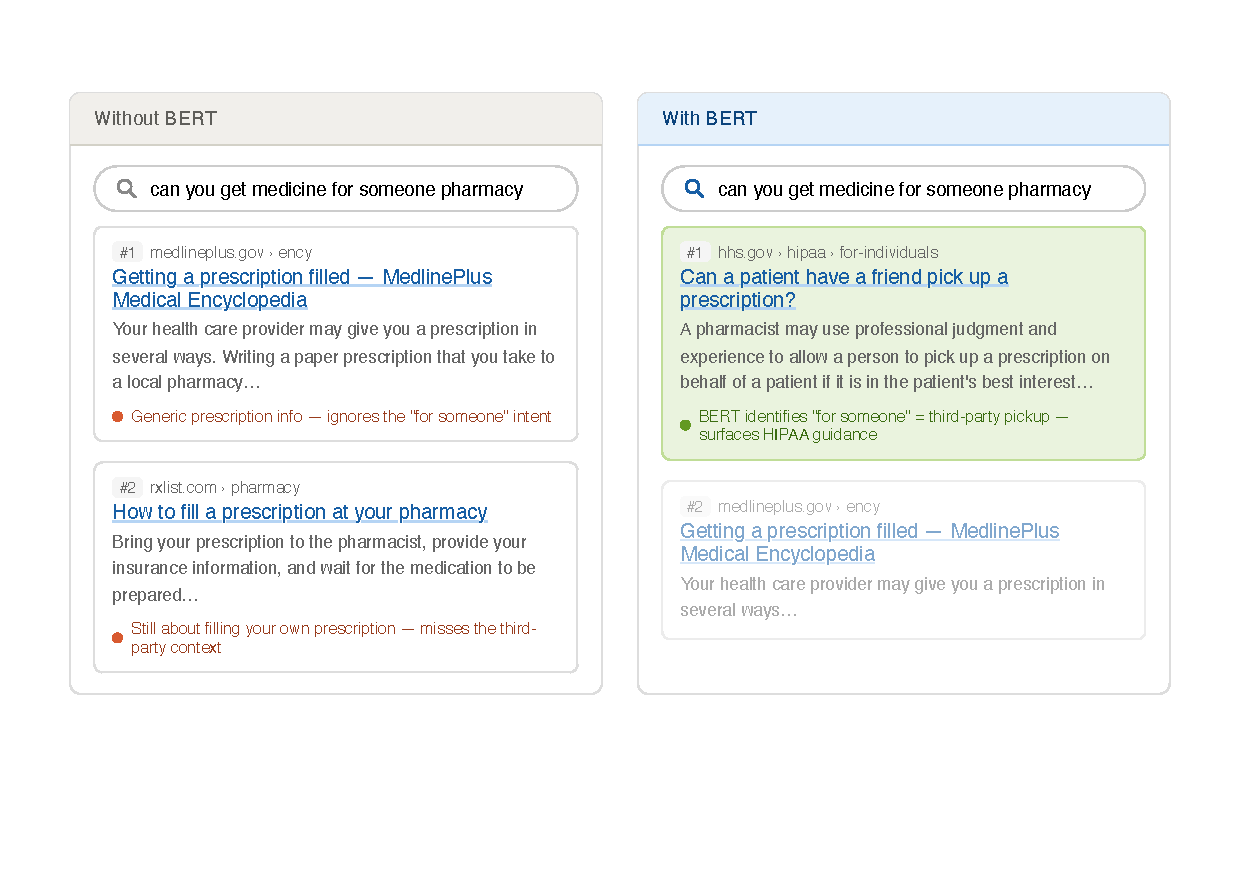
\includegraphics[trim=1cm 3cm 1cm 1.5cm, clip, width=0.90\textwidth]{figures/pharmacy.pdf}
  \caption{\textbf{Close-up of BERT Contextual Understanding.} Detailed view of the third-party intent resolution for pharmacy pickup queries.}
  \label{fig:pharmacy-zoom}
\end{figure}

A second example involves the query \emph{``Can you get medicine for someone
pharmacy''}.  Earlier systems surfaced general information about filling
prescriptions, overlooking the phrase \emph{``for someone''} which signals a
third-party pickup scenario.  \bert{}'s contextualisation correctly identifies
this intent, ranking results from authoritative health-policy sources that directly
address whether a pharmacist may dispense medication to a proxy.  These examples
demonstrate that even fine-grained syntactic relationships---which static keyword
matching cannot capture---are correctly resolved through \bert{}'s deep bidirectional
representations.

\subsection{Question Answering}
\label{subsec:qa}

Extractive question answering requires the model to locate a contiguous span of text
within a given passage that answers a posed question.  \bert{} addresses this as a
\emph{span extraction} task: the question and the context paragraph are concatenated
as \texttt{[CLS] Question [SEP] Context [SEP]}, and two linear layers predict the
start and end token indices of the answer span~\cite{devlin2019bert}.

Consider the following context passage: \emph{``The BERT-Large model is a powerhouse
of natural language processing.  It consists of 24 transformer layers and 16 attention
heads.  BERT-Large features 340 million parameters, allowing it to understand complex
nuances in human language.''}  Given the question \emph{``How many parameters does
BERT-Large have?''}, \bert{} assigns the highest start-position probability to the
token \emph{340} and the highest end-position probability to the token
\emph{million}, extracting the correct answer span \emph{``340 million''}.  This
behaviour arises because the cross-attention between the question tokens and the
context tokens guides the model towards the semantically relevant passage fragment.
On the Stanford Question Answering Dataset~(SQuAD~2.0), \bert{} achieved
state-of-the-art performance at the time of publication, surpassing human-level
accuracy on the held-out test set~\cite{rajpurkar2018know}.

\subsection{Named Entity Recognition}
\label{subsec:ner}

\begin{figure}[H]
  \centering
  % trim= left bottom right top 
  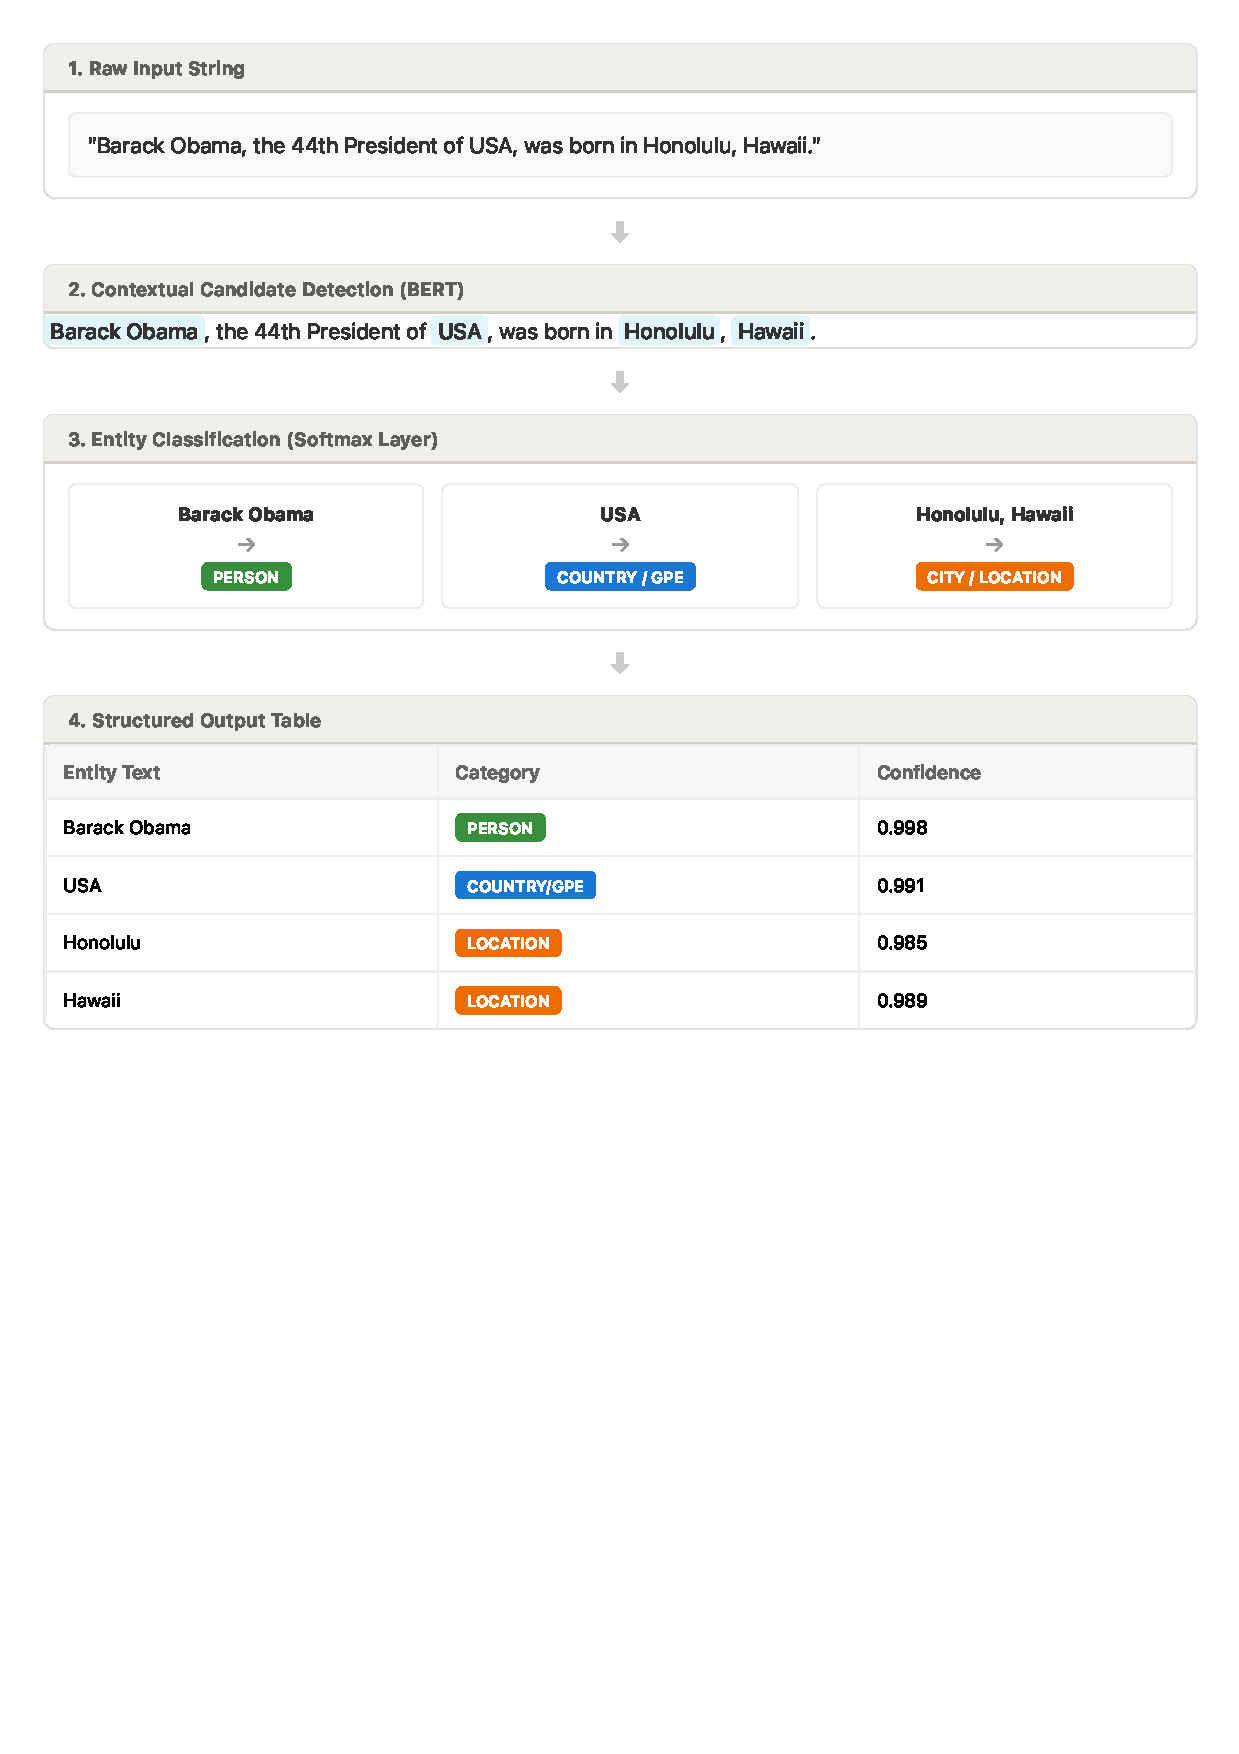
\includegraphics[trim=0cm 11cm 0cm 0.5cm, clip, width=0.90\textwidth]{figures/nerPipeline.pdf}
  \caption{\textbf{Four-Stage Named Entity Recognition (NER) Pipeline.} The diagram illustrates the transition from (1)~raw input strings to (2)~contextual candidate detection via \bert{}, followed by (3)~token-level classification into categories such as \textbf{Person}, \textbf{GPE}, and \textbf{Location}, and finally (4)~the consolidation of labels into a structured output table.}
  \label{fig:ner-pipeline-stages}
\end{figure}

Named Entity Recognition~(NER) is a token-level sequence labelling task in which the
model assigns a category label to each token in a sentence.  Common entity categories
include Person, Organisation, Location, Geopolitical Entity~(GPE), and Date/Time
expressions.  \bert{} approaches NER by appending a token-level classification head
atop the contextual encoder; the representation of each subword token is independently
passed through a softmax layer to produce a label~\cite{devlin2019bert}.

The pipeline can be described in four stages.  First, the raw input string---for
example, \emph{``Barack Obama, the 44th President of USA, was born in Honolulu,
Hawaii.''}---is tokenised and fed to the encoder.  Second, the model exploits
contextual signals to identify candidate entities; the phrase \emph{Barack Obama}
is highlighted as a named entity by virtue of its proper-noun characteristics and
surrounding syntactic structure.  Third, each detected entity is assigned its most
probable label: \emph{Barack Obama} $\rightarrow$ \textbf{Person}, \emph{USA}
$\rightarrow$ \textbf{Country/GPE}, and \emph{Honolulu, Hawaii} $\rightarrow$
\textbf{City/Location}.  Fourth, the labelled entities are collated into a structured
output table, which downstream applications can directly consume for information
extraction or knowledge-graph construction.


% ============================================================
%  Section: Limitations of BERT
% ============================================================

\section{Limitations of BERT}
\label{sec:limitations}

Despite its transformative impact, \bert{} is not without significant limitations.
Understanding these shortcomings is essential both for deploying \bert{} responsibly
and for motivating the extensive body of successor work that followed its
release~\cite{rogers2020primer}.


\begin{figure}[H]
  \centering
  % trim= left bottom right top 
  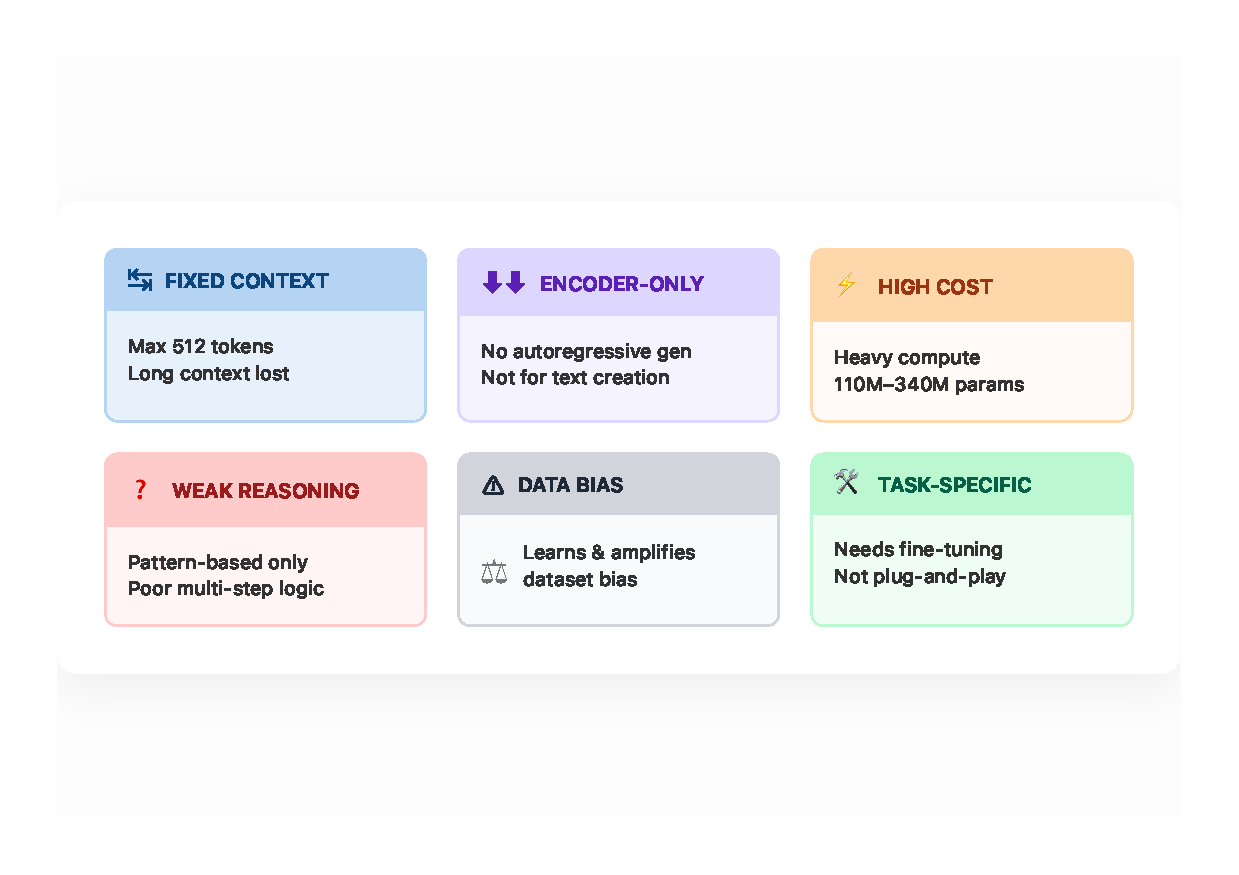
\includegraphics[trim=1cm 3cm 1cm 4cm, clip, width=0.90\textwidth]{figures/limitation.pdf}
  \caption{\textbf{Limitations of BERT.} Fixed context window, encoder-only design, high computational cost, weak reasoning ability, inherited data bias, and dependence on task-specific fine-tuning.}
  \label{fig:bert-limitations}

\end{figure}


\begin{enumerate}
  \item \textbf{Fixed context window.}  \bert{} operates on sequences of at most
        512 tokens.  Documents exceeding this limit must be truncated or chunked,
        which breaks cross-segment dependencies and can degrade performance on
        long-document tasks such as legal contract analysis or scientific paper
        summarisation.

  \item \textbf{Encoder-only architecture---no text generation.}  Because \bert{}
        is a \emph{bidirectional encoder}, it is architecturally incapable of
        auto-regressively generating text.  Tasks requiring open-ended generation,
        such as machine translation, abstractive summarisation, or dialogue,
        require decoder-equipped architectures (e.g., GPT, T5,
        BART)~\cite{lewis2019bart}.

  \item \textbf{Computational cost.}  \bert{}-Base contains 110 million parameters
        and \bert{}-Large 340 million.  Both require substantial GPU memory and
        inference time, making real-time deployment in resource-constrained
        environments (e.g., on-device mobile applications) challenging without
        additional compression~\cite{sanh2019distilbert}.

  \item \textbf{Limited commonsense and logical reasoning.}  \bert{}'s pre-training
        objectives---Masked Language Modelling and Next Sentence Prediction---equip
        it with strong distributional semantics but do not explicitly train it to
        perform multi-step reasoning or apply world knowledge consistently.  This
        manifests as errors on tasks requiring numerical reasoning, causal inference,
        or structured commonsense knowledge~\cite{rogers2020primer}.

  \item \textbf{Inherited data bias.}  \bert{} is pre-trained on BookCorpus and
        English Wikipedia.  These corpora encode various societal biases pertaining
        to gender, race, and cultural perspective.  Studies have shown that \bert{}'s
        representations reflect and can amplify such biases, which raises ethical
        concerns in applications involving hiring, credit scoring, or content
        moderation~\cite{bender2021dangers}.
\item \textbf{Task-specific dependency.} \bert{} is not a general-purpose, out-of-the-box 
        solution. Its pre-training objective (masked language modeling) does not directly 
        align with most downstream tasks, requiring additional fine-tuning on labeled data 
        for each specific application. As a result, performance is highly dependent on 
        task-specific datasets and supervision, limiting transferability and increasing 
        deployment cost.
\end{enumerate}


% ============================================================
%  Section: What Came After BERT
% ============================================================

\section{What Came After BERT}
\label{sec:successors}

\bert{}'s introduction triggered an era of rapid architectural innovation aimed at
addressing each of its known limitations while preserving or extending its core
strengths.  The resulting family of models can be broadly categorised into three
groups: training-efficiency improvements, context and modelling extensions, and
deployment-friendly distillations.

\begin{figure}[H]
  \centering
  % trim= left bottom right top 
  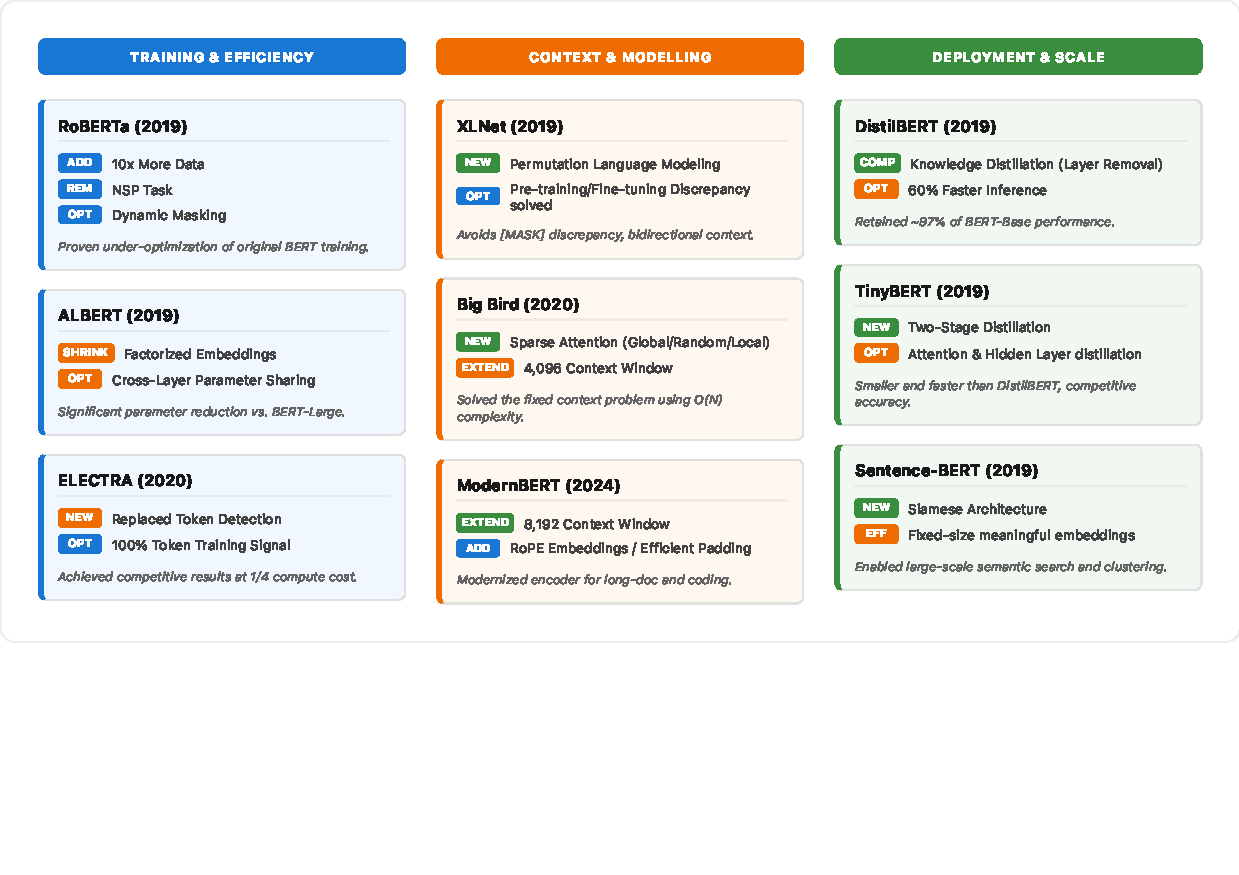
\includegraphics[trim=0cm 3cm 0cm 0cm, clip, width=0.90\textwidth]{figures/successors.pdf}
  \caption{\textbf{BERT Successors and Improvements.} Overview of key BERT-based models that address limitations in pre-training, model efficiency, context length, reasoning, and task adaptability.}
  \label{fig:bert-succesors}
\end{figure}

\subsection{Training and Efficiency Improvements}
\label{subsec:training-successors}

\textbf{RoBERTa}~(Robustly Optimised BERT Pre-training Approach, 2019) demonstrated
that \bert{}'s original training was substantially under-optimised.  By training on
ten times more data, removing the Next Sentence Prediction objective, and adopting
\emph{dynamic masking} (so that each training pass sees a different random mask),
Liu et al.\ achieved consistent improvements across all \textsc{GLUE} benchmarks
without any architectural change~\cite{liu2019roberta}.


\textbf{ALBERT}~(A Lite BERT, 2019) introduced two parameter-reduction techniques:
\emph{factorised embedding parameterisation}, which decouples the vocabulary
embedding size from the hidden layer size, and \emph{cross-layer parameter sharing},
where all Transformer layers share identical weights.  These changes reduced the
parameter count by up to 89\% relative to \bert{}-Large while maintaining competitive
accuracy~\cite{lan2019albert}.

\textbf{ELECTRA}~(Efficiently Learning an Encoder that Classifies Token Replacements
Accurately, 2020) replaced the MLM objective with a more sample-efficient
\emph{replaced-token detection} pre-training signal: a small generator network
corrupts the input and the main discriminator learns to identify which tokens were
replaced.  Because every token contributes a training signal (rather than only the
15\% masked tokens in standard MLM), ELECTRA reached \bert{}'s performance with
substantially less compute~\cite{clark2020electra}.

\subsection{Context and Modelling Extensions}
\label{subsec:context-successors}

\textbf{XLNet}~(2019) abandoned the masked-token paradigm in favour of
\emph{permutation language modelling}: by training the model to predict tokens in all
possible orderings of the input sequence, XLNet obtains bidirectional context without
the train--inference discrepancy introduced by \texttt{[MASK]}
tokens~\cite{yang2019xlnet}.


\textbf{BigBird}~(2020) introduced sparse attention mechanisms combining global, 
local, and random attention patterns to extend BERT's context window up to 4,096 
tokens while maintaining linear computational complexity. This design addresses 
BERT's fixed-context limitation, making it effective for long-document understanding 
and retrieval tasks~\cite{zaheer2020bigbird}.


\textbf{ModernBERT}~(2024) extended the context window to 8\,192 tokens through
Rotary Position Embeddings~(RoPE), incorporated efficient padding removal to avoid
unnecessary computation on padding tokens, and updated the architectural components
with current best practices.  These changes make ModernBERT competitive on long-document
retrieval and coding tasks while retaining the familiar encoder-only
paradigm~\cite{modernbert2024}.

\subsection{Deployment-Friendly Models}
\label{subsec:lightweight-successors}

\textbf{DistilBERT}~(2019) applied \emph{knowledge distillation} to compress
\bert{}-Base into a model with 40\% fewer parameters and 60\% faster inference,
retaining approximately 97\% of \bert{}'s performance on downstream
benchmarks~\cite{sanh2019distilbert}.

\textbf{TinyBERT}~(2019) applied a two-stage knowledge distillation approach 
to compress BERT into a smaller, faster model. By distilling both attention 
and hidden layers from the teacher model, TinyBERT achieves competitive 
accuracy with reduced parameters and inference time, enabling deployment 
in resource-constrained environments~\cite{jiao2019tinybert}.


\textbf{Sentence-BERT}~(SBERT, 2019) fine-tuned \bert{} with a Siamese network
architecture and a contrastive objective, producing \emph{fixed-size sentence
embeddings} that are semantically meaningful under cosine similarity.  This allows
large-scale semantic textual similarity, clustering, and information retrieval tasks
to be performed efficiently without the expensive cross-encoder inference required by
vanilla \bert{}~\cite{reimers2019sentencebert}.


% ============================================================
%  Section: Conclusion
% ============================================================

\section{Conclusion}
\label{sec:conclusion}

\bert{} represents a watershed moment in the history of natural language processing.
By introducing deep bidirectional pre-training via the Masked Language Model
objective, it resolved the fundamental limitation of unidirectional context that
constrained all prior pre-trained representations.  Its unified \emph{pre-train then
fine-tune} paradigm eliminated the need to design task-specific architectures from
scratch, establishing a blueprint that the entire field subsequently
adopted~\cite{devlin2019bert}.

Table~\ref{tab:before-after-bert} summarises the principal qualitative shifts that
\bert{} introduced, contrasting the capabilities of the NLP landscape before and
after its release.

\begin{table}[ht]
\centering
\caption{The evolution of NLP capabilities introduced by \bert{}.}
\label{tab:before-after-bert}
\renewcommand{\arraystretch}{1.4}
\begin{tabular}{p{0.44\textwidth} p{0.44\textwidth}}
\hline
\textbf{Before BERT} & \textbf{After BERT} \\ \hline
Unidirectional context (LSTMs, ELMo) & Full bidirectional context \\
Separate model trained per task & One backbone, many tasks \\
Shallow contextual signals & Deep contextual embeddings \\
Expensive training for each new task & Efficient fine-tuning on small data \\
Sequential processing (slow) & Parallel Transformer layers (fast) \\ \hline
\end{tabular}
\end{table}

The legacy of \bert{} extends far beyond its benchmark scores.  From its release in
2018 through RoBERTa and ALBERT in 2019, ELECTRA in 2020, and ModernBERT in 2022,
each successive model refined or extended \bert{}'s core ideas, collectively pushing
the frontier of language understanding.  Today, \bert{} and its successors underpin
production systems for web search, question answering, document classification, and
information extraction at global scale.  More broadly, \bert{} established the
Transformer encoder as the canonical architecture for language understanding---a
position it continues to hold, and one that has influenced the design of every major
language model released since~\cite{rogers2020primer, bender2021dangers}.